\subsubsection{Почему транзисторные ключи с инжекционным питанием имеют источник питания с самой маленькой ЭДС среди всех ключей? Какой?}

Ключ на интегрально-инжекторной логике представляет собой ключ, где в отличие от простого эмиттерного ключа резисторы (в частности Rб и Rк) заменены на генераторы стабильного тока, при этом все транзисторы могут быть запитаны от одного источника ЭДС с использованием горизонтального многоколлекторного транзистора.

Поясним сказанное на примере.

\begin{center}
	\begin{figure}[h!]
		\center{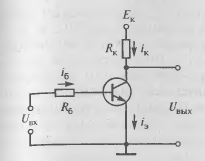
\includegraphics[scale=3]{iil/image001.png}}
		\caption{Простейший ключ}	
		\label{iil1}
	\end{figure}
\end{center}

 

\begin{center}
	\begin{figure}[h!]
		\center{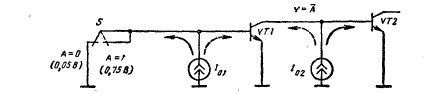
\includegraphics[scale=2]{iil/image003.png}}
		\caption{Инвертор на базе иил ключа}	
		\label{iil3}
	\end{figure}
\end{center}



В иил ключе не используются резисторы Rб и Rк, тратящие много времени и мощности. 

Вместо них используются источники питания. 

В левом положении ключа S, соответствующем уровню  лог. 0 (0.05 В) ток от генератора идет через ключ (транзистор , выполняющий роль ключа, аналогичный транзисторам VT1 и VT2) на землю. При этом транзистор VT1 заперт, потому что на его базу не подано напряжение, достаточное для отпирания ключа. Поэтому ток от генератора I2 идет на базу транзистора VT2 и переводит его в режим насыщения. Напряжение база-эмиттер такого транзистора около 0.75 В, что соответствует уровню лог. 1. Выходной сигнал можно снять с клеммы Y.

В правом положении ключа S ток I1 отпирает транзистор VT1, переводя его в режим насыщения. Условие такого перехода -- Biб$>$Iкнас выполнено. На схеме BI1$>$I2. При I1=I2 и B $>$ 1 это всегда выполняется. Напряжение между коллекторам и эмиттером выбранного насыщенного транзистора, как уже было сказано, 0.05 В. На клемме Y -- искомый нулевой сигнал.

В иил используются источники питания с самой низкой эдс среди всех ключей, потому что транзистор переходит в насыщение уже при напряжении Uбэ=0.75В. Резистор используется один -- в источнике питания, для его стабилизации. Поэтому, ЭДС источника -- около 1,15В. В других ключах необходимо большее эдс, потому что значительная часть напряжения теряется на Rб.

В частности, источник подключается так:

\begin{center}
	\begin{figure}[h!]
		\center{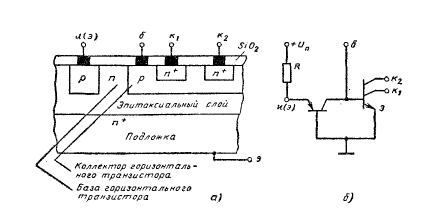
\includegraphics[scale=1.5]{iil/image005.png}}
		\caption{}	
		\label{iil5}
	\end{figure}
\end{center}



Применение:
\begin{center}
	\begin{figure}[h!]
		\center{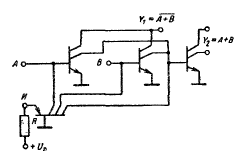
\includegraphics[scale=2]{iil/image007.png}}
		\caption{}	
		\label{iil7}
	\end{figure}
\end{center}

На этой схеме и схеме б) показано, что для запитывания иил ключа достаточно подключить источник эдс через резистор R к горизонтальному pnp транзистору. Он выдает на своем коллекторе (коллекторах) стабильный ток, от которых можно подать питание все имеющиеся в ней npn транзисторы, необходимое для их отпирания (насыщения) или запирания (перевода в режим отсечки).
